\chapter{Architecture du projet}

	\section{Arborescence du projet}

		Notre application est organisée de la manière suivante :


		\begin{figure}[H]
			\centering
			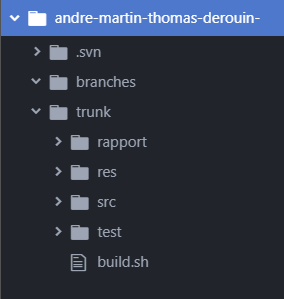
\includegraphics[width=0.5\textwidth, keepaspectratio]{img/racine.png}
		\end{figure}

		On y retrouve 4 dossiers et 1 fichier:

		\begin{description}
			\item [rapport:] Contient ce rapport sous latex
			\item [res:] Contient les ressources du jeu, c'est-à-dire l’image par défaut pour le taquin
			\item [src:] Contient le code source de l’application
			\item [test:] Contient le code se chargeant des tests unitaires
			\item [build.sh:] Fichier de compilation du taquin.
		\end{description}

		On notera en réalité la présence supplémentaire d'un dossier \textit{doc} contenant la Javadoc ainsi que d'un dossier \textit{dist} contenant le jar exécutable. Ceux-ci ne sont pas notés car ils sont générés avec le script de compilation.

		Le code source du projet est situé dans le chemin \textit{src/taquin/}. Il est constitué par :

		\begin{figure}[H]
			\centering
			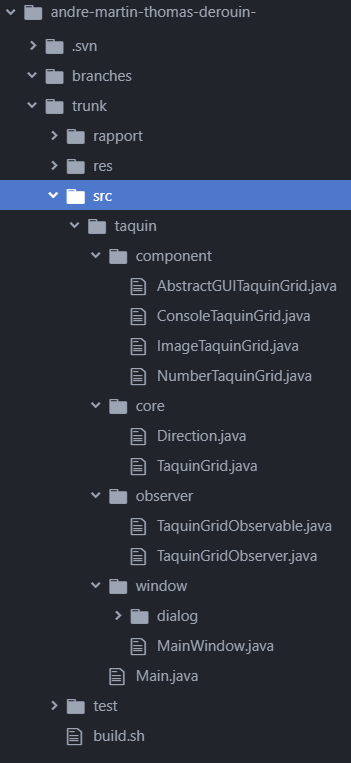
\includegraphics[width=0.5\textwidth, keepaspectratio]{img/detail.png}
		\end{figure}

		\begin{description}
			\item [component:] Contient les différents composants de l’application.
			\item [core:] Contient le cœur du jeu du taquin, non dépendant de l'affichage graphique, ainsi que la classe qui énumère les directions
			\item [observer:] Contient les classes relatives à l'implémentation du pattern Observer
			\item [window:] Contient les classes permettant de gérer ce qui se rapporte à la fenêtre de jeu et des boites de dialogues
			\item [Main.java:] Classe exécutable du projet.
		\end{description}

	\section{Mise en place du pattern MVC}

	Dans notre projet, il nous a été demandé d'utiliser le design pattern MVC. Il a été mis en place de la manière suivante:

	\begin{figure}[H]
		\centering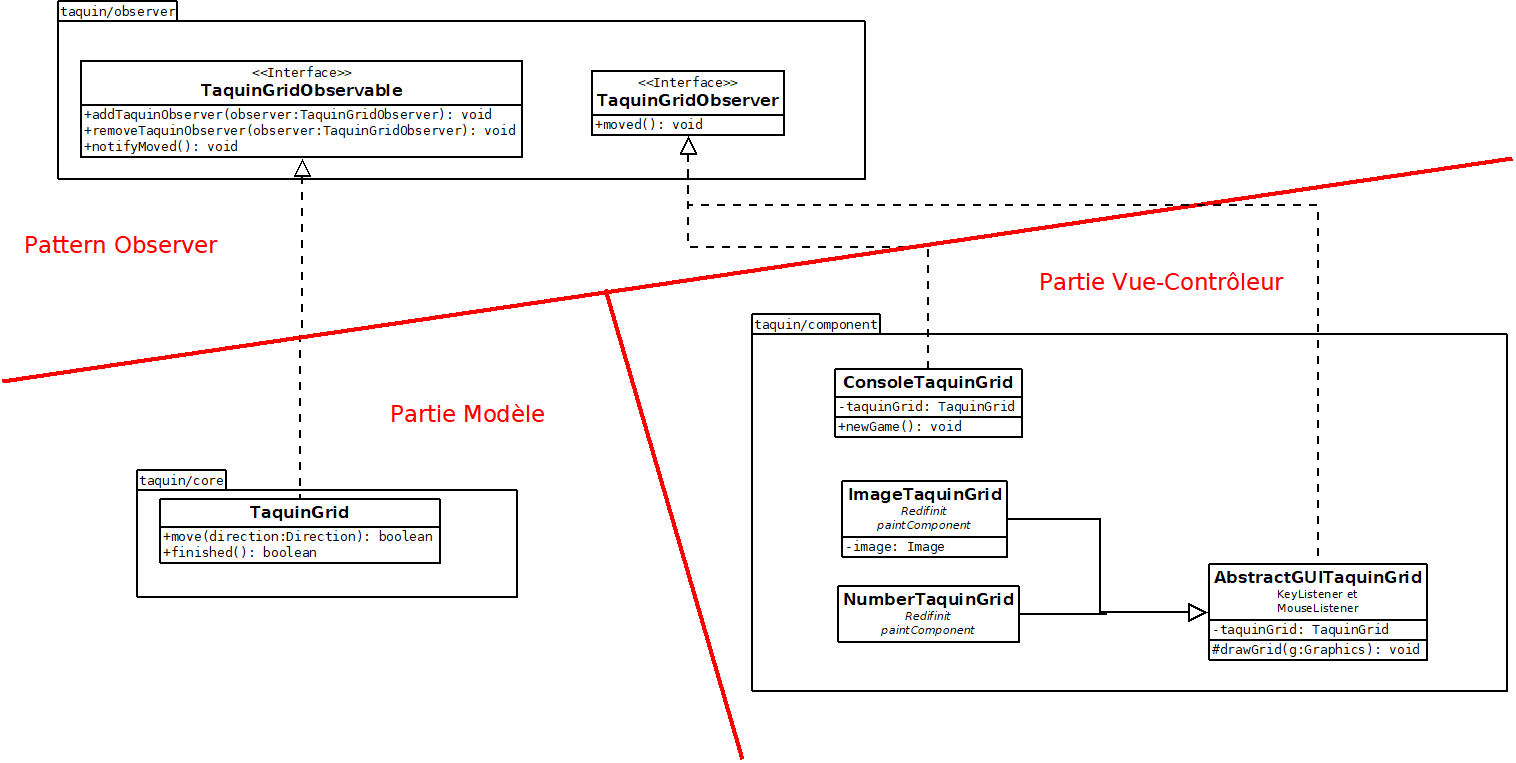
\includegraphics[width=1\textwidth, keepaspectratio]{img/diagramMVC.png}
		\caption{Notre tableau Trello}
		\label{Mise en place du M-VC}
	\end{figure}

	Nous avons la classe \textbf{TaquinGrid} qui est le modèle pour une grille de jeu. Tous les traitements sont donc absolument identiques peu importe la vue. On utilisera, par exemple; la même méthode pour déplacer une case peu importe qu'il s'agisse d'un affichage en console ou en fenêtre.

	Nous avons d'un autre coté, tout le package component, qui lui, contient les différentes vues de l'application qui jouent également le rôle de contrôleurs. Nous avons décidé de concevoir trois Vues-Contrôleurs différentes :

	\begin{itemize}
		\item [Pour le monde console:] Vue-Contrôleur représentée par la classe \textbf{ConsoleTaquinGrid}
		\item [Pour le mode image:]  Vue-Contrôleur représentée par la classe \textbf{ImageTaquinGrid}
		\item [Pour le mode nombre:]  Vue-Contrôleur représentée par la classe \textbf{NumberTaquinGrid}
	\end{itemize}

	Pour être plus précis, la classe mère \textbf{AbstractGUItaquinGrid} est un contrôleur parent aux classes \textbf{ImagetaquinGrid} et \textbf{NumbertaquinGrid}. Ces deux dernières ne font que de redéfinir la manière dont nous affichons l'information grâce à la méthode \textit{void paintComponent(Graphics)}
